
%(BEGIN_QUESTION)
% Copyright 2011, Tony R. Kuphaldt, released under the Creative Commons Attribution License (v 1.0)
% This means you may do almost anything with this work of mine, so long as you give me proper credit

Predict the effects of the steam supply pressure suddenly decreasing in this steam reforming system.  Assume all loop components are properly configured, that the controller is well-tuned, and that a significant amount of time has passed since the supply pressure changed.  Compare these conditions with what they were before the process change: 

$$\includegraphics[width=15.5cm]{i01707x01.eps}$$

\begin{itemize}
\item{} Steam valve will: {\it open up} further, {\it close down} more, or {\it remain in the same position} 
\vskip 10pt
\item{} Methane valve will: {\it open up} further, {\it close down} more, or {\it remain in the same position} 
\end{itemize}

\underbar{file i01707}
%(END_QUESTION)





%(BEGIN_ANSWER)

\begin{itemize}
\item{} Steam valve will: {\bf open up further}
\vskip 5pt
\item{} Methane valve will: {\bf remain in the same position}
\end{itemize}

%(END_ANSWER)





%(BEGIN_NOTES)

{\bf This question is intended for exams only and not worksheets!}.

%(END_NOTES)


